\chapter{Preliminary Literature review}\label{review}
Bed topography is one of the most crucial boundary conditions that influences ice flow and loss from the Antarctic Ice Sheet (AIS)~\cite{Morlighem_2020}. Bed topography datasets are typically generated from airborne radar surveys, which are sparse and unevenly distributed across the Antarctic continent. Interpolation schemes—such as those used in Bedmap ice bed, surface and thickness gridded datasets for Antarctica~\cite{Lythe_2001, Fretwell_2013, Pritchard_2025}, or BedMachine~\cite{Morlighem_2017}—to ``gap fill'' these sparse datasets yield bed topography estimates that have uncertainties of multiple hundreds of metres in elevation~\cite{Morlighem_2020} which propagate through simulations of AIS evolution under climate change~\cite{Castleman_2022}. Given the logistical challenges of accessing large parts of Antarctica, there is a crucial need for alternative approaches that integrate diverse and possibly more spatially complete data streams – including satellite data.

\section{Approaches to Bed Topography Reconstruction}
To address the critical gap in understanding subglacial conditions, my research goal is to develop a method that combines forward and inverse modelling, leveraging high-resolution satellite surface data, significantly improve bed topography estimates in regions where direct radar measurements are sparse.
The generation of gridded bed topographies in Antarctica is based on two primary modelling approaches to infer subglacial bed topography and its influence on ice dynamics, these are classified as forward and inverse models. 

Forward models aim to understand how different bed properties influence ice flow. These often generate interpolated gridded topography using geostatistical techniques like kriging~\cite{Mackie_2020} and are valuable for investigating how uncertainties in the bed can impact outcomes like simulated ice mass loss. Forward models can generally be classed as elevation-preserving or texture-preserving (the bed's geostatical properties are mantained), their fundamental limitation is that they rely on assumptions about the bed conditions rather than direct observation, exploring possibilities rather than determining the actual topography. 

Inverse models involve methods that assimilate other data sources and work by inferring bed properties, such as topography or basal slipperiness, from surface observations like ice elevation and velocity. Techniques like control method inversion~\cite{deRydt_2013} and 4dvar assimilation minimise mismatches between observed and simulated data, on the other hand mass conservation approaches use physical laws to reconstruct the bed, especially where measurements are sparse~\cite{Morlighem_2017, Morlighem_2020}. Despite their power, these methods face significant challenges. Variational approaches often require regularisation to prevent non-physical results and over-fitting~\cite{Morlighem_2024}, and time-dependent methods like 4dvar are computationally expensive. Probabilistic methods such as Markov Chain Monte Carlo (MCMC) are powerful for quantifying uncertainty but remain too computationally intensive~\cite{Morlighem_2024} for large-scale models.

Another issue is that it is still uncommon for methods to systematically quantify the relationship between bed topography and its morphometric landscape statistics. Studies that measure the statistics report them as continuous fields and terrain types are assigned to specific regions rather than to individual cells, with each parameter described qualitatively. Siegert et al.~\cite{Siegert_2004} define three bed roughness groups across named areas of East Antarctica, and Rippin et al.~\cite{Rippin_2014} assign three terrain types to the areas of their survey. Numerical thresholds have been published for single parameters, and Jordan et al.~\cite{Jordan_2017} divide the Hurst exponent at 0.5 and 0.75 to define low, medium and high roughness categories, but no scheme applies thresholds to a combination of axes per analysed cell. For published classified maps, each cell is often assigned to one class with no margin reported alongside it: Ockenden et al.~\cite{Ockenden_2026} map the Antarctic bed into five landscape classes on 50~km cells, and their accompanying data release~\cite{Ockenden_2025_data} records each assignment without a confidence interval or an alternative class. In addition, ambiguity in landscape class is often only acknowledged as a caveat or analysed under a qualitative lens of multiple interpretations but it is not rigorously quantified, so a published class cannot be read alongside the alternatives that the measurement might still admit. That absence of margins makes such maps vulnerable to survey artefacts, since local roughness measurement bias due to radar migration status or uneven coverage can move a measurement across a boundary without leaving any trace. This often results in averaged regimes that in turn fail to capture the true continuum of the subglacial landscape.

In chapter~\ref{progress}, I introduce Observational Data Spectral Analysis (ODSA), a physically informed framework for quantifying Antarctic subglacial landscape characteristics and classifying bed morphology into archetypes for ice sheet modelling. The landscape classification provides an empirical foundation for the generation of structurally realistic synthetic bed topographies. ODSA operates on the along-track picks published with Bedmap3 instead of a gridded product, the tracks are visible in Fig.~\ref{fig:Bedmap+Ockenden_map}, measuring the survey data directly and avoiding the interpolation we described earlier. 
\begin{figure}[H]
    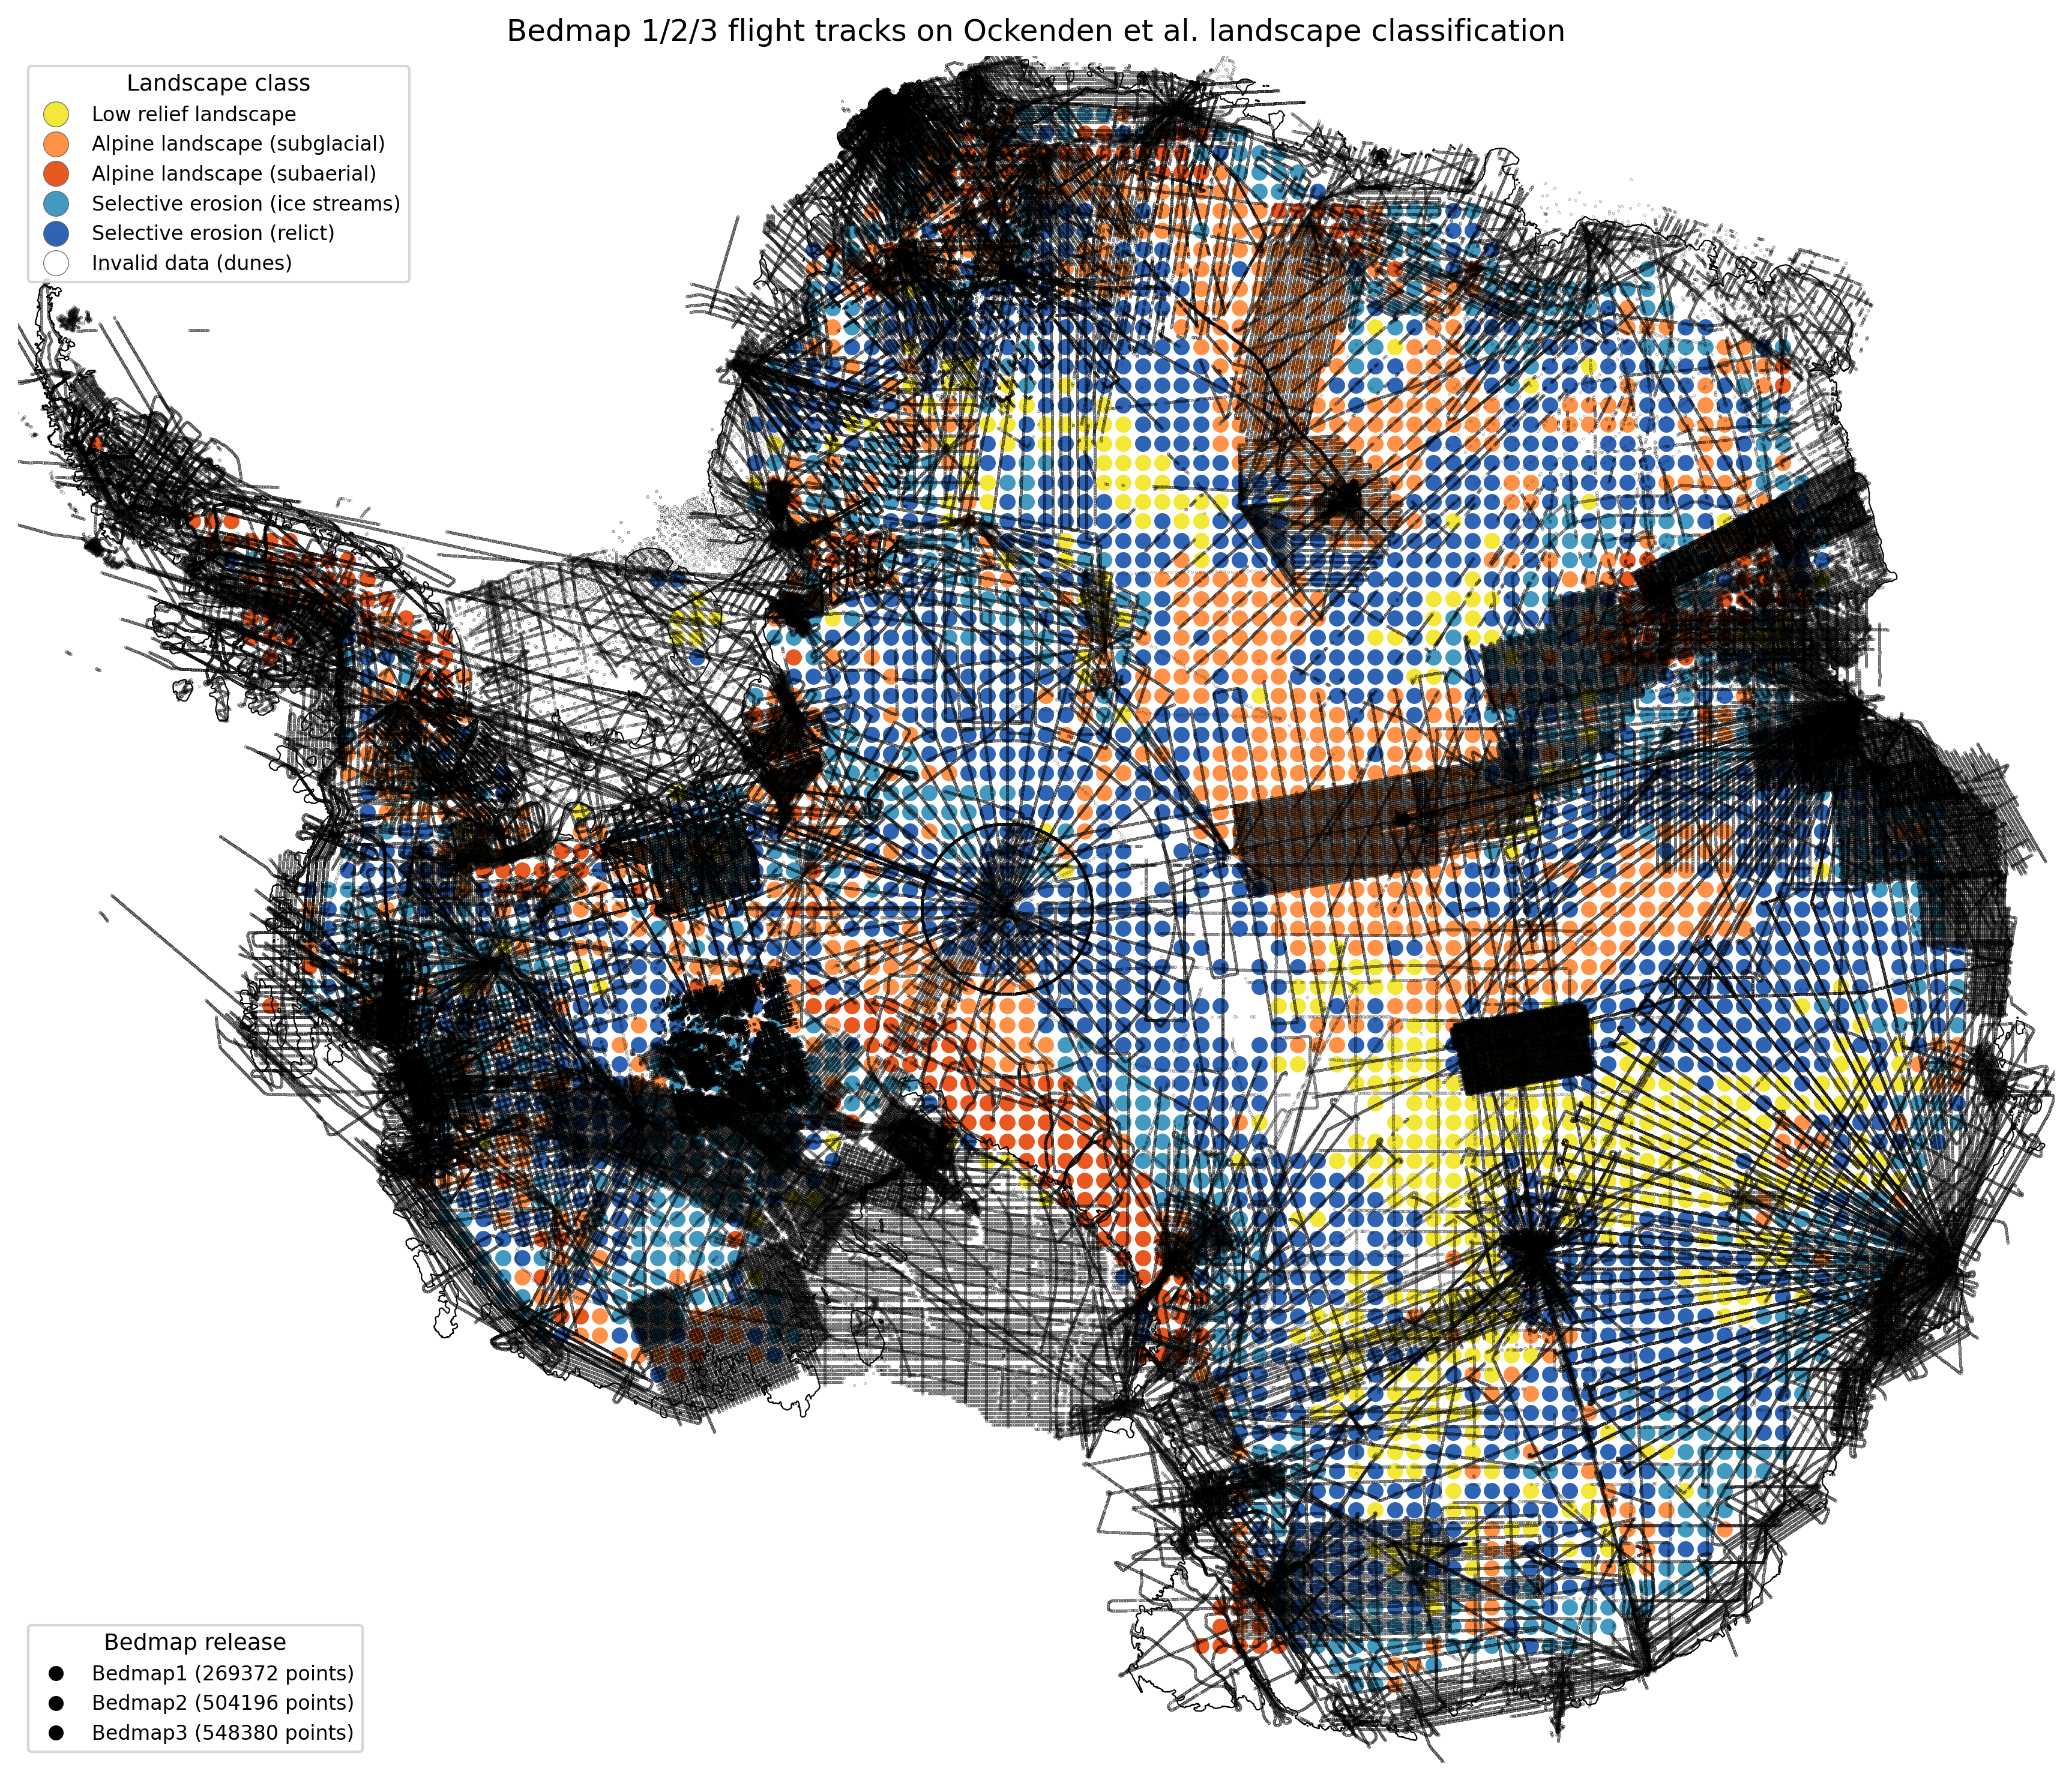
\includegraphics[scale=0.45]{figures/bedmap123_on_ockenden.png}
    \caption{Bedmap1, Bedmap2 and Bedmap3 along-track survey points (black) over the continental landscape classification map by Ockenden et al.~\cite{Ockenden_2026} (coloured cells, cells masked as invalid data (dunes) are drawn white). We reproduce the classification from the published metric grids~\cite{Ockenden_2025_data} on 50~km cells.
    The point counts in the legend show the number of subsampled plotted points rather than published picks. ODSA operates on these along-track data, so the figure shows the sampling available to us across a continental landscape classification.} 
    \label{fig:Bedmap+Ockenden_map}
\end{figure}

\section{From Signal Transfer to Tractable Inversion}\label{theoretical_frameworks}

This project aims to develop a framework to connect observable surface features to the subglacial bed below, ensuring that the governing physics of ice sheet flow are respected. To do this, my work focuses in utilising surface-bed transfer functions.

The core principle behind a transfer function is that the ice sheet acts as a physical filter, modifying the expression of bed features as they propagate to the surface. The work by Budd~\cite{Budd_1970} established that ice preferentially dampens short-wavelength bed undulations while features with a wavelength approximately $3.3\times$ the ice thickness are most clearly expressed at the surface~\cite{Budd_1970}. This process also introduces a phase lag, and can be described mathematically using frequency-dependent transfer functions. More recent studies have built directly on this foundation. For instance, Gudmundsson and Raymond~\cite{Gudmundsson_2008} refined the transfer function concept for ice streams, and Ockenden et al.~\cite{Ockenden_2023} applied it in reverse, using full-Stokes transfer functions to invert high-resolution satellite observations of surface elevation and velocity to infer bed properties. These studies collectively establish that the physical relationship between the bed and the surface provides a viable pathway for subglacial mapping.

Despite the success of these approaches, their practical application has been limited by simplifying assumptions about ice physics. A primary limitation is the reliance on a linear (Newtonian) ice rheology, where stress is directly proportional to the strain rate (i.e., a ``constant viscosity''). This assumption is often utilised to make the inversion mathematically tractable, but it contrasts with the widely accepted non-linear Glen's Flow Law, where the stress exponent is typically $n \approx 3$ or even $n = 4$. Nevertheless. the choice of rheology is a critical control on the bed-to-surface signal transfer; a non-linear rheology ($n = 4$) produces significantly different surface expressions compared to a linear one ($n = 1$), and by largely ignoring non-linear rheology and complex basal sliding conditions, past inversion methods have introduced uncertainties and may not be robustly applicable across all dynamic regimes of the ice sheet.

The critical opportunity lies in the exploiting the vast wealth of underutilised high-resolution satellite surface observations including NASA's ITS\_LIVE~\cite{itslive} velocities and REMA elevations~\cite{REMA}. My approach with BedSAT will harness these data streams by building upon established transfer function theory while addressing the fundamental limitation that has restricted past approaches: the mathematical intractability of non-linear ice physics.

BedSAT will connect surface observations with bed topography using more realistic rheological assumptions ($n = 4$) and complex sliding conditions, rather than the simplified linear physics commonly used by traditional inversions. The key step to making this process tractable is Physics-Informed Machine Learning (Physics-ML), which solves the computational bottleneck that has forced previous methods to rely on unrealistic simplifications. By leveraging NVIDIA PhysicsNeMo—designed to blend governing physics (PDEs) with training data~\cite{NVIDIA_NeMo_2025}—BedSAT can learn the non-linear mapping between surface expressions and bed topography without linearising the physics. This approach transforms what was previously computationally intractable into a fast, accurate inverse solver.
Through an iterative process where initially inverted bed topography is integrated into forward models for progressive refinement, BedSAT will deliver physically consistent reconstructions validated against independent datasets. This represents a fundamental advance: where previous methods had to choose between physical realism and computational feasibility, Physics-ML enables both simultaneously.

